\section{Risikoanalyse}
\begin{figure}[H]
	\centering
	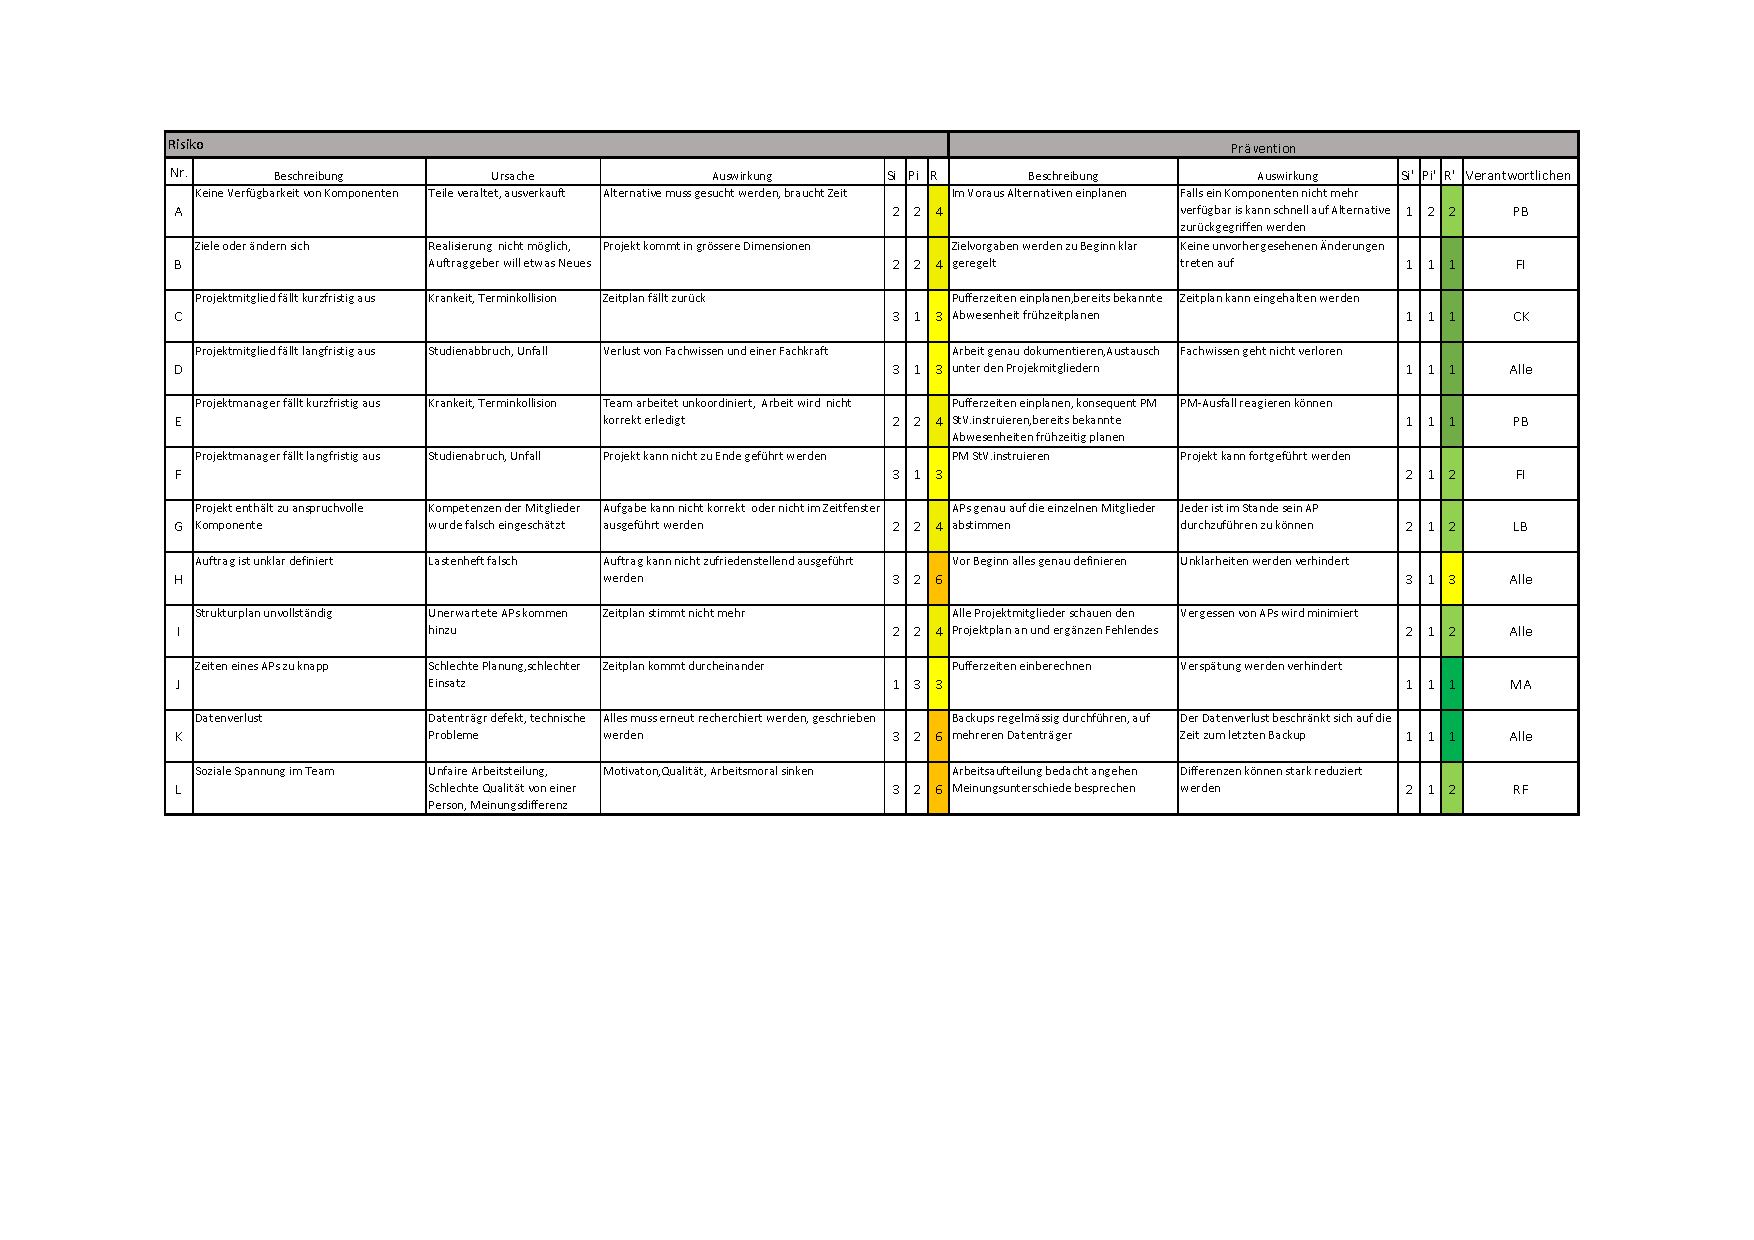
\includegraphics[width=10cm]{Risikoanalyse.pdf}
	\label{fig:Risikoanalyse}
\end{figure}

\newpage

Um auf Risiken vorbereitet zu sein, macht man eine Risikotabelle. In dieser werden die möglichen Ge- fahren aufgelistet und bereits Präventionsmassnahmen genannt, um sowohl die Eintrittswahrscheinlich- keit(Pi), als auch die Auswirkungen(Si) zu minimieren. Auf der Risikomap werden zudem alle Gefahren mit und ohne Prävention graphisch dargestellt.

\begin{figure}[H]
	\centering
	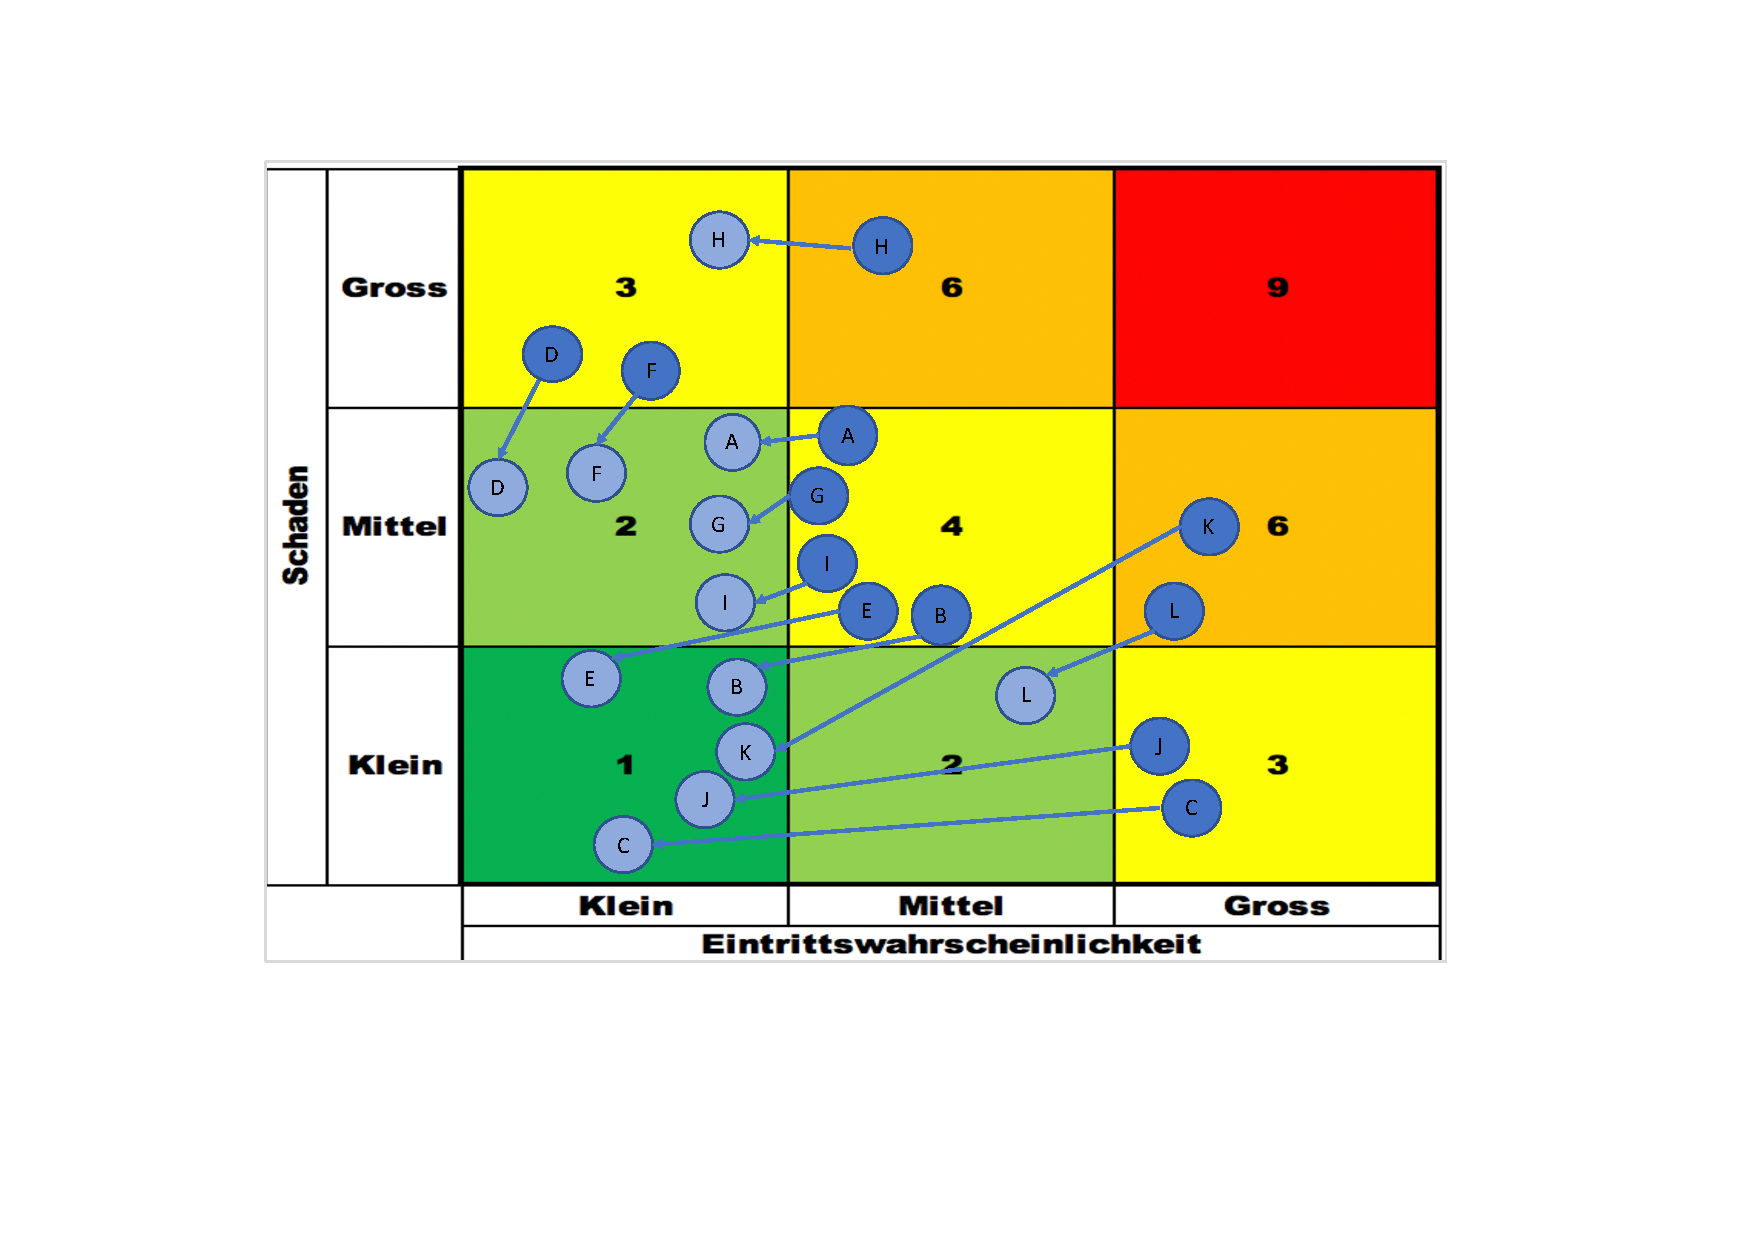
\includegraphics[width=10cm]{Risikotab.pdf}
	\label{fig:Risikodiagramm}
\end{figure}

\begin{figure}[H]
	\centering
	\includegraphics[width=10cm]{Risikotabelle}
	\label{fig:Tabelle}
\end{figure}
A Keine Verfügbarkeit von Komponenten
B Ziele ändern sich
C Projektmitglied fällt kurzfristig aus
D Projektmitglied fällt langfristig aus
E Projektmanager fällt kurzfristig aus
F Projektmanager fällt langfristig aus
G Projekt enthält zu anspruchvolle Komponente
H Auftrag ist unklar definiert
I Strukturplan unvollständig
J Zeiten eines APs zu knapp
K Datenverlust
L Soziale Spannung im Team
